\chapter{Interacting Quantum Field Theory}
\setcounter{chapter}{4}
\section{Introduction and examples}
Theories discussed so far are Klein-Gordon theory with spin $0$ 
\begin{align}\lag_{KG} = \frac{1}{2}\partial_\mu\phi\partial^\mu\phi - \frac{m^2}{2}\phi^2\end{align}
and Dirac theory spin $\frac{1}{2}$ 
\begin{align}\lag_D = \bar{\psi}(i\slashed{\partial} - m) \psi \end{align}

There is also $\lag_{EM} = -\frac{1}{4}F_{\mu\nu}F^{\mu\nu}$ with $F_{\mu\nu} = \partial_\mu A_\nu - \partial_\nu A_\mu$ for a massless vector filed. Its quantisation gives photon.

One thing they have in common is they are all quadratic in the fields. As a result:
\begin{itemize}
	\item linear field equations
	\item exact quantisation
	\item multi-particle states without scattering or interaction
	\item linear Fourier decomposition, no momentum changes
\end{itemize}

To have an interacting theory with scattering, need higher powers in the field in the Lagrangians. A few examples are following
\paragraph{Scalar $\phi^4$ theory}
\begin{align*}
	\lag = \lag_{KG} + \frac{\lambda}{4!} \phi^4
\end{align*}
need positive sign $\lambda > 0$ for a stable theory, otherwise classical energy can be arbitrarily negative.

Equation of motions
\begin{align*}
	(\partial^2+ m ^2) \phi = -\frac{\lambda}{3!} \phi^3
\end{align*}
is non-linear, cannot be solved by Fourier decomposition.

\paragraph{Yukawa-theory}
\begin{align*}
	\lag = \lag_{KG} + \lag_{D} - g \bar{\psi}\psi \phi
\end{align*}
is originally developed as a theory for nuclear forces with $\psi$ nucleon, $\phi$ pion. In the Standard Model it is similar to interactions in Higgs mechanism.
\paragraph{Quantum Electrodynamics (QED)}
\begin{align*}
	\lag = \lag_{EM} + \lag_{D} - eA_\mu \bar{\psi} \gamma^\mu \psi
\end{align*}
describes electrons, their antiparticles positrons and photons.

\paragraph{Yang-Mills theory}
generalises $\lag_{EM}$ with terms like $A^4$ or $A^2 \partial A$
\paragraph{Scalar QED}
describes pions and photons
\begin{align*}
	\begin{split}
		\lag &= \lag_{EM} + D_\mu \phi D^\mu\phi^* - m^2 |\phi|^2 \\
			 &= \lag_{EM} + \partial_\mu\phi\partial^\mu\phi^* - m^2 \phi\phi^* + ie A_\mu(\phi\partial^\mu\phi^* - \phi^* \partial^\mu\phi) + e^2 A_\mu A^\mu \phi\phi^*
	\end{split}
\end{align*}
\paragraph{Remarks}
\begin{itemize}
	\item Interaction terms in $H_\text{int} = \int \dd^3x \ham_\text{int} = - \int\dd^3x\lag_\text{int}$ always involves products of fields at the same point $\pmb{x}$. It ensures causality, no "instant at a distance".
	\item There are no derivative interactions. These may complicate quantisation as $$\pi(\pmb{x}) = \frac{\partial\lag}{\partial(\partial_0 \phi(\pmb{x}))}$$
	\item Why are we taking the examples above? There must be zillions of theories (Lagrangians)? \\
			We have the criterion of \textbf{renormalizability}. Note the mass dimensions of fields;
			\begin{align*}
				[S] = 1 \, \text{so} \, [\lag] = [M]^4 \, \Rightarrow [\phi] = [M] ,\, [\psi] = [M]^{\frac{3}{2}} ,\, [A_\mu] = [M]
			\end{align*}
			So in all the interaction terms indicated above, the coupling constant $\lambda$, e, g are all \textbf{dimensionless}!\\
			Can add $-\frac{\mu}{3!}\phi^3$ to the $\phi^4$ theory. This leads to $[\mu] = [M]$ and all these generate renormalizable interactions. \\
			All higher interaction terms require coupling constants of \textbf{negative} mass dimension, e.g. $G\bar{\psi}\psi\bar{\psi}\psi$ and then $[G] = [M]^{-2}$. These are non-renormalizable and create trouble when performing higher-order calculation in perturbation theory.
			(with energy cut-off; corrections $~G\Lambda^2$, $\Lambda \rightarrow \infty$)
		\item We haven't quantised the photon yet. The reason is that its is a vector field, i.e. 4 degrees of freedom, but photon has just $2$ physical polarisation states. It is linked to gauge symmetry and complicates quantisation somewhat.
\end{itemize}
\section{The interaction picture}
Consider the $\phi^4$ theory, 
\begin{align}
\lag_{int} = -\frac{\lambda}{4!} \phi(x)^4
\end{align}
Hamiltonian $H = H_0 + H_{int}$ with 
\begin{align}
	H_0 &= \int\dd^3 x \left\{ \frac{1}{2}\pi^2(x) + \frac{1}{2}(\pmb{\nabla}\phi)^2 + \frac{1}{2}m^2\phi^2 \right\}\\
	H_\text{int} &= -\int\dd^3x \lag_\text{int} = \frac{\lambda}{4!}\int\dd^3x \phi^4 
\end{align}

Interaction picture means that \textit{operators} evolve in time using $H_0$ (only), in particular 
\begin{align}
	\phi_I(t,\pmb{x}) = e^{iH_0t}\phi(\pmb{x})e^{-iH_0t}
\end{align}

Time-dependence of the free field obeys classical equation of motion $\left(\partial^2+m^2 \right)\phi_I(t,\pmb{x}) = 0$. Solution in terms of Fourier modes as before:
\begin{align}
	\phi_I(t,\pmb{x}) = \int \frac{\dd^3 p}{(2\pi)^3\sqrt{2E_p}} (a^I_{\pmb{p}}e^{-ipx} + a^{I\,\dagger}_{\pmb{p}}e^{+ipx})
\end{align}
as in the free theory with standard commutation relations $[a^I_{\pmb{p}}, a^{I\,\dagger}_{\pmb{p}}] = (2\pi)^3\delta^{(3)}(\pmb{p}-\pmb{p}')$. The state satisfying $a^I_p \ket{0} = 0$ is the vacuum of the free, non-interacting theory.

Relation between interaction and Schrödinger picture states:
\begin{align}
	\ket{\psi_I(t)} = e^{iH_0t}{\ket{\psi_S(t)}}
\end{align}
Schrödinger equation becomes: 
\begin{align}
	i\frac{\partial}{\partial t}\ket{\psi_S} &= (H_0 + H_\text{int})\ket{\psi_S} \notag\\
	\text{LHS} &= i \frac{\partial}{\partial t} \left( e^{-iH_0t}\ket{\phi_I} \right) = H_0 e^{-iH_0t}\ket{\phi_I} + e^{-iH_0t}i\frac{\partial}{\partial t}\ket{\phi_I} \notag\\
	\text{RHS}														&= \left(H_0 + H_\text{int}\right)e^{-iH_0t}\ket{\phi_I} \notag\\
	\Rightarrow i\frac{\partial}{\partial t}\ket{\phi_I} &= e^{iH_0t}H_\text{int} e^{-iH_0t} = H_I(t)\ket{\phi_I} \label{math:int-schr}
\end{align}
with $H_I$ interaction Hamiltonian in the interaction picture. Clearly
\begin{align}
	H_I = \frac{\lambda}{4!}\int\dd^3x\phi_I^4(x) \notag
\end{align}

What is the solution of~\ref{math:int-schr} for the time evolution of $\ket{\phi_I(t)}$? Define time-evolution operator in the interaction picture.
\begin{align}
	\ket{\phi_I(t)} &= U(t,t_0)\ket{\phi_I(t_0)}\label{math:int-schr2}\\
	\text{with} \; U(t,t_0) &= e^{iH_0(t-t_0)}e^{-iH(t-t_0)} 
\end{align}

With~\ref{math:int-schr} and~\ref{math:int-schr2}:
\begin{align}
	i\frac{\partial}{\partial t} U(t,t_0) = H_I(t)U(t,t_0)
\end{align}

To solve with boundary conditions $U(t_0, t_0) = \id$. The formal solution is then:
\begin{align}
	U(t,t_0) = 1 - i \int_{t_0}^t \dd t' H_I(t')U(t',t_0) \notag
\end{align}

Substitute back in and we get:
\begin{align*}
	U(t,t_0) = 1- i \int_{t_0}^t \dd t' H_I(t') + (-i)^2 \int_{t_0}^t \dd t' \int^{t'}_{t_0} \dd t'' H_I(t') H_I(t'') + \dots
\end{align*}

$H_I$ inside the integral is automatically time-ordered. Ranges of integration is not. 

\begin{figure}[ht]
	\centering
	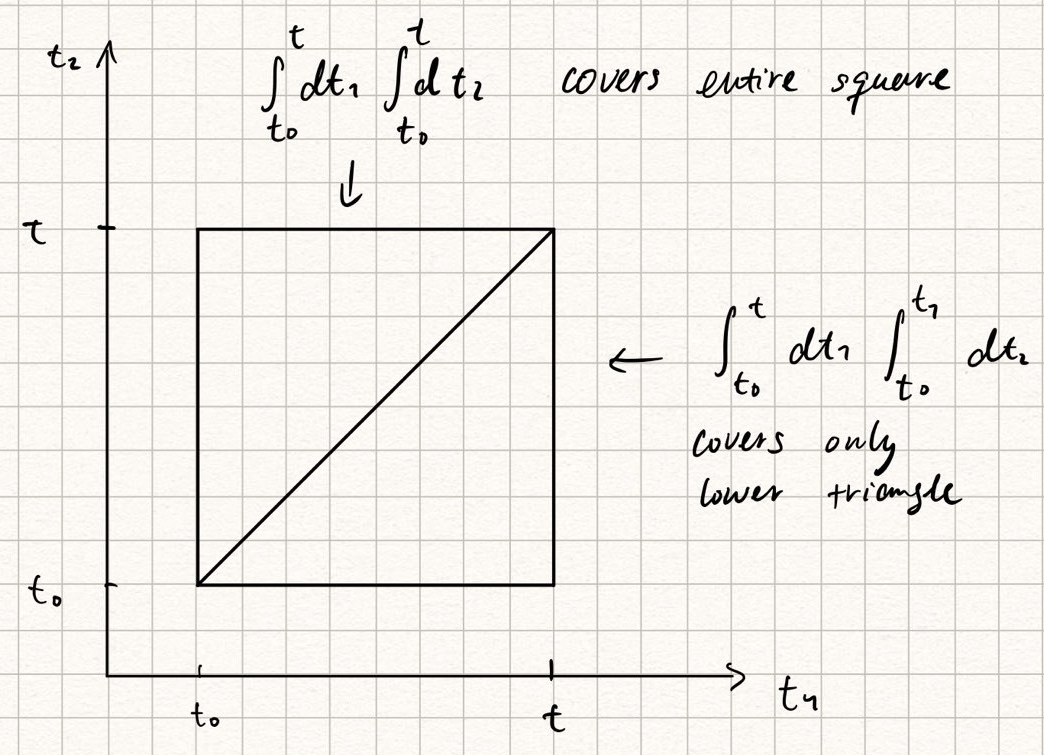
\includegraphics[width=0.65\linewidth]{4-2-triangle.jpg}
	\caption{Time ordering}
	\label{fig:4-2-triangle}
\end{figure}

Upper triangle has the wrong time order. We are going to "repair" it by hand.
\begin{align}
	U(t,t_0) &= 1-i\int_{t_0}^t \dd t' H_I(t') + \frac{(-i)^2}{2} \int_{t_0}^t \dd t' \int^{t}_{t_0} \dd t'' T(H_I(t') H_I(t'')) + \dots \notag\\
			 &= \sum_{n=0}^{\infty} \frac{(-i)^n}{n!}\int_{t_0}^t \dd t_1 \dots \int_{t_0}^t \dd t_n T(H_I(t_1) \dots H_I(t_n))  \notag\\
			 &= T \exp{-i\int_{t_0}^t \dd t' H_I(t') }
\end{align}

It is interesting for scattering to transition into asymptotic state for $t \rightarrow \infty$
\begin{align}
	S = \lim_{t \rightarrow \infty} U(t,-t) &= T \exp{-i \int_{-\infty}^\infty \dd t H_I(t)} \\
	 &\stackrel{\phi^4}{=} T \exp{-i\int \dd^4 x \frac{\lambda}{4!} \phi_I^4(x)} \notag
\end{align}
Both $U$ and $S$ are formally unitary

Composition law for time evolution operator
\begin{align}
	U(t_2, t_0) = U(t_2, t_1) U(t,t_0) = U(t_2, t_1) U(t_0, t_1)^\dagger
\end{align}

\subsection{Scattering amplitudes and the S-matrix}
Take $\ket{i}$ the initial (multi-particle) state and $\ket{f}$ the final (multi-particle) state. Time evolution of $\ket{i}$ then is
$$\lim_{t\rightarrow\infty} U(t,-t) \ket{i} = S \ket{i}$$

Probability that $\ket{i}$ evolves into $\ket{f}$ is proportional to the squared "\textbf{S-matrix element}"
\begin{align}
	\left|	\braket{f,\, t\to \infty | i, t\rightarrow - \infty}\right|^2 = \left| \braket{f|S|i} \right|^2 = \left| S_{fi} \right|^2
\end{align}

The non-trivial part of the S-matrix is the T-matrix:
\begin{align}
	S_{fi} \defeq \delta_{fi} + iT_{fi}
\end{align}

Use momentum conservation (from translation invariance) to define matrix element
\begin{align}
	S_{fi} = \delta_{fi} + i(2\pi)^4 \delta^{(4)}(p_f - p_i) M_{fi}
\end{align}
$M_{fi}$ measures "genuine scattering" from $\ket{i}$ to $\ket{f}$.

How are we going to calculate correlation functions in the interacting theory:
\begin{align*}
	\braket{\Omega |  \ T \phi(x)\phi(y) | \Omega}	
\end{align*}
or more generally $\braket{\Omega | T \phi(x_1)\phi(x_2)\dots | \Omega}$? Here $\ket{\Omega}$ is the vacuum/ground state of the interacting theory $\ham$ (in contrast to $\ket{0}$ is the ground state of $\ham_0$) and $\phi(x)$ the Heisenberg operators.

Ignore $\ket{\Omega} \neq \ket{0}$ for the moment saying that we want to study the time evolution from the vacuum at $t\rightarrow - \infty$ to $t \rightarrow + \infty$. So rewriting in terms $\phi_I(x)$, assuming $x^0 > y^0$ for now:
\begin{align}
	\braket{0 | U(\infty, x^0) \phi_I(x^0)  U(x^0, y^0) \phi_I(y^0)U(y^0, -\infty) | 0}  = \braket{0|T(\phi_I(x)\phi_I(y)S)|0}
\end{align}
still holds if $x^0 < y^0$ because of $T$.

Now $\ket{\Omega} \neq \ket{0}$: this can be taken care of by dividing out the time evolution of the (free) vacuum $\braket{0|S|0}$, so
\begin{align}
	\braket{\Omega | T(\phi(x)\phi(y))|\Omega} &= \frac{\braket{0 | T(\phi_I(x)\phi_I(y)S)|0}}{\braket{0|S|0}} \\
	&\stackrel{\phi^4}{=} 
	\frac{\braket{0 | T {\phi_I(x)\phi_I(y)\exp{-i\int\dd^4x' \frac{\lambda}{4!}\phi^4(x')}}| 0}}
	{\braket{0 | T {\exp{-i\int\dd^4x' \frac{\lambda}{4!}\phi^4(x')}}| 0}
}\notag
\end{align}
Proof can be found in Peskin. It will also be illustrated practically later ("vacuum bubbles").

Perturbation theory is viable when $\lambda$ (or some other coupling) is "small" and then expands $U(t,t_0)$ or $S$ in powers of $\lambda$.

\section{Wick's theorem}
From now on drop the subscript for interaction picture fields $\phi_I(x) \rightarrow \phi(x)$ for convenience.

Want to calculate stuff like $\braket{0 | T\phi(x_1)\dots\phi(x_n)S | 0}$ in perturbation theory, e.g.\ at order $\lambda^n$.  
\begin{align}
\frac{1}{n!} \left( -i\frac{\lambda}{4!} \right)^n \int \dd^4 y_1 \dots \dd^4 y_n \braket{0 | T\phi(x_1)\dots\phi(x_n)\phi^4(y_1)\dots\phi^4(y_n) | 0}
\end{align}

We know $\braket{0 | T\phi(x_1)\phi(x_2) | 0 } $ is the Feynman propagator!

Recall \textbf{normal ordering} with $\phi(x) = \phi^+(x) + \phi^-(x)$
\begin{align}
	:\phi^+ \phi^-: = :\phi^- \phi^+: = \phi^- \phi^+
\end{align} 
where
\begin{align}
\phi^+ &= \int \frac{\dd^3 p}{(2\pi)^3} \frac{1}{\sqrt{2E_{\pmb{p}}}} a_{\pmb{p}} e^{-ip\cdot x} \\
	\phi^- &= \int \frac{\dd^3 p}{(2\pi)^3} \frac{1}{\sqrt{2E_{\pmb{p}}}} a^\dagger_{\pmb{p}} e^{+ip\cdot x}
\end{align}
Wick's theorem expresses time-ordered products in terms of normal-ordered ones. Then it is easy to take vacuum expectation values, as $\braket{0 | :\phi(x_1)\dots\phi(x_n):|0} = 0$

Take two fields and $x^0 > y^0$:
\begin{align*}
	T \phi(x)\phi(y) &= \phi(x)\phi(y) = \left(\phi^+(x)+\phi^-(x)\right)\left(\phi^+(y)+\phi^-(y)\right) \\
	&= \phi^+(x)\phi^+(y) + \phi^-(x)\phi^-(y) + \phi^-(x) \phi^+(y) + \phi^-(x) \phi^+(y) + [\phi^+(x), \phi^-(y)] \\
	&= :\phi(x)\phi(y): + [\phi^+(x),\phi^-(y)]
\end{align*} 

Particularly for $y^0 > x^0$: 
\begin{align}
	T\phi(x)\phi(y) = :\phi(x)\phi(y): + [\phi^+(y),\phi^-(x)] \notag
\end{align}

Thus altogether: 
\begin{align}
	T\phi(x)\phi(y) = :\phi(x)\phi(y): + D_f(x-y)
\end{align}
as $\Theta(x^0 - y^0) [\phi^+(x), \phi^-(y)] + \Theta(y^0 - x^0) [\phi^+(y), \phi^-(x)] = D_F(x-y)$.

Worth noting that $D_F(x-y)$ is still a c-number, not operator (yet). Thus it can be pulled out of any matrix element or expectation value.

We now define "contraction":
\begin{align}
	\contraction[1ex]{}{\phi}{(x_1)}{\phi}	\phi(x_1) \phi(x_2) = D_F(x_1-x_2)
\end{align}

Thus we can remove the fields from the product leaving only the propagators:
\begin{align}
	T\phi(x)\phi(y) = :\phi(x)\phi(y): +  \contraction[1ex]{}{\phi}{(x)}{\phi}	\phi(x) \phi(y)
\end{align}

General form of \textbf{Wick's theorem} for arbitrary number of fields
\begin{align}
	T\phi(x_1)\dots \phi(x_n) = :\phi(x_1)\dots \phi(x_n):	 + :\left( \text{sum over all possible contractions} \right):
\end{align}

Example with four fields:
\begin{align*}
	T(\phi_1 \phi_2 \phi_3 \phi_4) &= :\phi_1 \phi_2 \phi_3 \phi_4: \\
								   & + \contraction{}{\phi_1}{}{\phi_2} \phi_1 \phi_2 :\phi_3 \phi_4: + \contraction{}{\phi_1}{}{\phi_3} \phi_1 \phi_3 :\phi_2 \phi_4: + \contraction{}{\phi_1}{}{\phi_4} \phi_1 \phi_4 :\phi_2 \phi_3: +  \contraction{}{\phi_2}{}{\phi_3} \phi_2 \phi_3 :\phi_1 \phi_4: + \contraction{}{\phi_2}{}{\phi_4} \phi_2 \phi_4 :\phi_1 \phi_3: + \contraction{}{\phi_3}{}{\phi_4} \phi_3 \phi_4 :\phi_1 \phi_2: \\
	&+ \contraction{}{\phi_1}{}{\phi_2} \phi_1 \phi_2 \contraction{}{\phi_3}{}{\phi_4}\phi_3 \phi_4 + \contraction{}{\phi_1}{}{\phi_3} \phi_1 \phi_3 \contraction{}{\phi_2}{}{\phi_4}\phi_2 \phi_4 + \contraction{}{\phi_1}{}{\phi_4} \phi_1 \phi_4 \contraction{}{\phi_2}{}{\phi_3}\phi_2 \phi_3
\end{align*}

Thus 
\begin{align*}
	\braket{0 | T \left(\phi_1 \phi_2 \phi_3 \phi_4 \right) | 0} = D_F (x_1 - x_2) D_F(x_3 - x_4) + D_F (x_1 - x_3) D_F(x_2 - x_4) + D_F (x_1 - x_4) D_F(x_2 - x_3) 
\end{align*}
which can be visually represented as
\begin{center}
\begin{tikzpicture}[scale=1, transform shape]
	\begin{feynman}
		\vertex (x1) {$x_1$};
		\vertex [below=of x1] (x2) {$x_2$};
		\vertex [right=of x1] (x3) {$x_3$};
		\vertex [below =of x3] (x4) {$x_4$};
		\diagram*{
			(x1) -- (x2),
			(x3) -- (x4),
		};
	\end{feynman}	
\node at (2,-0.8) {$+$};
\end{tikzpicture}
\begin{tikzpicture}[scale=1, transform shape]
	\begin{feynman}
		\vertex (x1) {$x_1$};
		\vertex [below=of x1] (x2) {$x_2$};
		\vertex [right=of x1] (x3) {$x_3$};
		\vertex [below =of x3] (x4) {$x_4$};
		\diagram*{
			(x1) -- (x3),
			(x2) -- (x4),
		};
	\end{feynman}	
\node at (2,-0.8) {$+$};
\end{tikzpicture}
\begin{tikzpicture}[scale=1, transform shape]
	\begin{feynman}
		\vertex (x1) {$x_1$};
		\vertex [below=of x1] (x2) {$x_2$};
		\vertex [right=of x1] (x3) {$x_3$};
		\vertex [below =of x3] (x4) {$x_4$};
		\diagram*{
			(x1) -- (x4),
			(x3) -- (x2),
		};
	\end{feynman}	
\end{tikzpicture}
\end{center}

%%%%%%%% 15.05.2019 %%%%%%%
Proof of the general theorem by \textit{induction} in the number of fields (see exercise). The idea is to suppose it is true for $\phi_2 \dots \phi_m$, $x^0_1 > x^0_{k>1}$. Then 
\begin{align*}
	T\phi_1 \phi_2 \dots \phi_m &= (\phi^+_{1} + \phi^-_{1})T\phi_2 \dots \phi_m \\
								& = (\phi^+_{1} + \phi^-_{1}) [:\phi_2 \dots \phi_m: + :\text{contractions}:]
\end{align*}
$\phi^-_1$ can stay as it is part of $(:\phi_1 \phi_2 \dots \phi_m:)$. But $\phi^+_1$ needs to be commuted past all $\phi^-_1$ operators, giving rise to additional contractions $\contraction{}{\phi_1}{}{\phi_2} \phi_1\phi_2$.

\paragraph{Consequences}
\begin{itemize}
	\item $n = 2k+1, \, k \in \N$
		\[
		\braket{0 | T \phi_1 \dots \phi_m | 0} = 0
		\]
	\item $n = 2k, \, k \in \N$	
		\[
			\braket{0 | T \phi_1 \dots \phi_m | 0} = \sum_{\text{pairing of fields}} D_F(x_{i_1}-x_{i_2})\dots D_F(x_{i_{m-1}}-x_{i_m})
		\]
\end{itemize}

\subsection{Wick's theorem and the S-Matrix}
Apply Wick's theorem to correlation functions $\braket{0 | T (\phi_1 \dots \phi_m ) S | 0}$ n-th term in the perturbative expansion of $S$ with $\phi(x_1) \defeq \phi_1$.
\begin{align*}
   \frac{1}{n!} \left(\frac{-i\lambda}{4!}\right)^n \int \dd^4 y_1 \dots \dd^4 y_n \braket{0 | T ( \phi_1 \dots \phi_m  \phi^4(y_1) \dots \phi^4(y_n) ) | 0}
\end{align*}

\paragraph{Example with $m=4 ,\, n=1$}
\begin{align*}
	-\frac{i\lambda}{4!} &\int \dd^4 x \braket{0 | T \phi_1 \phi_2 \phi_3 \phi_4 \phi^4(x) | 0} \\
	= &-\frac{i\lambda}{4!}  \int \dd^4 x \braket{0 |
		\acontraction{}{\phi_1}{\phi_2 \phi_3 \phi_4}{\phi}
		\acontraction[2ex]{\phi_1}{\phi_2}{\phi_3 \phi_4 \phi(x)}{\phi}
		\bcontraction[1ex]{\phi_1\phi_2}{\phi_3}{\phi_4 \phi(x) \phi(x)}{\phi}
		\bcontraction[2ex]{\phi_1 \phi_2 \phi_3}{\phi_4}{\phi(x) \phi(x) \phi(x)}{\phi}
		\phi_1 \phi_2 \phi_3 \phi_4 \phi(x) \phi(x) \phi(x) \phi(x) 
		| 0} + \text{23 permutations} \\
	& -\frac{i\lambda}{4!}  \int \dd^4 x  \braket{0 | 
		\acontraction{}{\phi_1}{}{\phi_2}
		\acontraction{\phi_1\phi_2}{\phi_3}{\phi_4}{\phi}
		\bcontraction{\phi_1 \phi_2 \phi_3}{\phi_4}{\phi(x)}{\phi}
		\acontraction{\phi_1 \phi_2 \phi_3 \phi_4 \phi(x)\phi(x)}{\phi}{(x)}{\phi}
		\phi_1 \phi_2 \phi_3 \phi_4 \phi(x)\phi(x)\phi(x)\phi(x) 
		| 0} + \text{11 permutations} + \text{5 similar} \\
	& -\frac{i\lambda}{4!}  \int \dd^4 x  \braket{0 | 
		\contraction{}{\phi_1}{}{\phi_2}\phi_1 \phi_2 \contraction{}{\phi_3}{}{\phi_4}\phi_3 \phi_4 \contraction{}{\phi}{(x)}{\phi}\phi(x)\phi(x)\contraction{}{\phi}{(x)}{\phi}\phi(x)\phi(x) 
	| 0} + \text{2 permutations} + \text{2 similar} \\
		=& -i\lambda \int \dd^4 x D_F(x_1 - x) D_F(x_2 - x) D_F(x_3 - x) D_F(x_4 - x) \\
	&- \frac{i\lambda}{2} D_F(x_1 - x_2) \int \dd^4 x D_F(x_3 - x) D_F(x_4 - x) D_F(x-x)+ \text{5 similar} \\
	& -\frac{i\lambda}{8} D_F(x_1 - x_2) D_F(x_3 - x_4) \int \dd^4 x D_F(x-x) + \text{2 similar}
\end{align*}
Permutation means permutation of $\phi(x)$ and similar means exchanging external states $\phi_i, \,i \in \{1,2,3,4 \}$ without changing the shape of diagram. Note that the pre-factors of the integrals are called \textit{symmetry factor}. The number of permutations of first diagram is equivalent to arrangement of 4 elements
$$\frac{4!}{4!}=1$$ 
The permutations of second digram are to link two internal points to external ones and the rest external points can link to either of internal one.
$$\begin{pmatrix} 4 \\ 2 \end{pmatrix}\cdot 2 \cdot \frac{1}{4!}= \frac 1 2$$ 
There are only three ways to permute a vacuum bubble
$$\frac{3}{4!}=\frac 1 8$$

To be represented in Feynman diagrams:
\begin{center}
\begin{tikzpicture}[scale=1, transform shape]
	\begin{feynman}
		\vertex (x1) {$x_1$};
		\vertex (x2) at (2,0) {$x_2$};
		\vertex (x3) at (0,-2){$x_3$};
		\vertex (x4) at (2,-2) {$x_4$};
		\vertex (x) at (1,-1);
		\diagram*{
			(x1)--(x)--(x2),
			(x3)--(x)--(x4),
		};
	\end{feynman}
	\node at (1,-1.3) {$x$};
	\node at (2.4,-1) {+};
\end{tikzpicture}
\begin{tikzpicture}[scale=1, transform shape]
	\begin{feynman}
		\vertex (x1) {$x_1$};
		\vertex (x2) at (2,0) {$x_2$};
		\vertex (x3) at (0,-2){$x_3$};
		\vertex (x4) at (2,-2) {$x_4$};
		\vertex (x) at (1,-1.5);
		\vertex (y) at (1,-0.8);
		\diagram*{
			(x1)--(x2),
			(x3)--(x)--(x4),
			(x) --[half left] (y) --[half left] (x),
		};
	\end{feynman}
	\node at (1,-1.8) {$x$};
	\node at (3.4,-1) {and 5 similar + };
\end{tikzpicture}
\begin{tikzpicture}[scale=1, transform shape]
	\begin{feynman}
		\vertex (x1) {$x_1$};
		\vertex (x2) at (2,0) {$x_2$};
		\vertex (x3) at (0,-2){$x_3$};
		\vertex (x4) at (2,-2) {$x_4$};
		\vertex (x)  at (2.5,-1);
		\vertex (y) at (2.5,-0.3);
		\vertex (z) at (2.5,-1.7);
		\diagram*{
			(x1)--(x2),
			(x3)--(x4),
			(x) --[half left] (y) --[half left] (x);
			(x) --[half left] (z) --[half left] (x);
		};
	\end{feynman}
	\node at (2.5,-1.2) {$x$};
	\node at (4,-1) {and 2 similar};
\end{tikzpicture}
\end{center}

In fact $D_F(x-x) = D_F(0)$ diverges!

\paragraph{Example with $m=0, \, n=1$} vacuum diagram
\begin{align*}
	& -\frac{i\lambda}{4!} \int \dd^4 x \braket{0 | T \phi^4(x) | 0} \\
	& = -\frac{i\lambda}{8} [D_F(0)]^2 \int \dd^4 x \\
	& 
\begin{tikzpicture}[scale=1, transform shape]
	\begin{feynman}
		\vertex (x)  at (0.5,-1);
		\vertex (y) at (0.5,-0.3);
		\vertex (z) at (0.5,-1.7);
		\diagram*{
			(x) --[half left] (y) --[half left] (x);
			(x) --[half left] (z) --[half left] (x);
		};
	\end{feynman}
	\node at (0,-1) {$=$};
	\node at (0.5,-1.2) {$x$};
\end{tikzpicture}
\end{align*}

\paragraph{Example: 2nd order S-matrix term}
\begin{align*}
	\frac{1}{2!} \left(\frac{-i\lambda}{4!} \right)^4 \int \dd^4 x\dd^4 y \braket{0 | T \phi_1 \phi_2 \phi_3 \phi_4 \phi^4(x) \phi^4(y) | 0}
\end{align*}
It has many contractions and some of the fully connected ones are of the type
there are 
\begin{align*}
	& (4\times 3) [\text{choose } \phi(x)]  \times (4\times 3) [\text{choose } \phi(y)]  \times 2 [\text{x-y-cont.}] \times 2 (\text{x-y-symm.}) + 2 \text{ similar, exchanging external points} \\
	 &= \frac{(-i\lambda)^2}{2} \int \dd^4 x \dd^4 y D_F(x_1 - x) D_F(x_2 -x )D_F(x_3-y)D_F(x_4-y) [D_F(x-y)]^2 + \text{2 similar} \\
	 &
	\begin{tikzpicture}[scale=1, transform shape]
	\node at (-0.5, -1) {$=$};
	\begin{feynman}
		\vertex (x1) {$x_1$};
		\vertex (x2) at (2,0) {$x_2$};
		\vertex (x3) at (0,-2){$x_3$};
		\vertex (x4) at (2,-2) {$x_4$};
		\vertex (x) at (1,-0.6);
		\vertex (y) at (1,-1.4);
		\diagram*{
			(x1)-- (x) --(x2),
			(x3)-- (y) --(x4),
			(x) --[half left] (y) --[half left] (x),
		};
	\end{feynman}
	\node at (1,-0.35) {$x$};
	\node at (1,-1.65) {$y$};
	\node at (2.5, -1) {$+$};
\end{tikzpicture}
\begin{tikzpicture}[scale=1, transform shape]
	\begin{feynman}
		\vertex (x1) {$x_1$};
		\vertex (x2) at (2,0) {$x_2$};
		\vertex (x3) at (0,-2){$x_3$};
		\vertex (x4) at (2,-2) {$x_4$};
		\vertex (x) at (0.6,-1);
		\vertex (y) at (1.4,-1);
		\diagram*{
			(x1)-- (x) --(x3),
			(x2)-- (y) --(x4),
			(x) --[half left] (y) --[half left] (x),
		};
	\end{feynman}
	\node at (0.4,-1) {$x$};
	\node at (1.6,-1) {$y$};
	\node at (2.5, -1) {$+$};
\end{tikzpicture}
\begin{tikzpicture}[scale=1, transform shape]
	\begin{feynman}
		\vertex (x1) {$x_1$};
		\vertex (x4) at (2,0) {$x_4$};
		\vertex (x3) at (0,-2){$x_3$};
		\vertex (x2) at (2,-2) {$x_2$};
		\vertex (x) at (0.6,-1);
		\vertex (y) at (1.4,-1);
		\diagram*{
			(x1)-- (x) --(x3),
			(x2)-- (y) --(x4),
			(x) --[half left] (y) --[half left] (x),
		};
	\end{feynman}
	\node at (0.4,-1) {$x$};
	\node at (1.6,-1) {$y$};
\end{tikzpicture}
\end{align*}

\paragraph{Symmetry factors}
A lot of the contractions eliminate the factors $\frac{1}{n!} \left(\frac{1}{4!}\right)^n$ in the denominators; the $\frac{1}{4!}$ was chosen to yield 
\begin{tikzpicture}[scale=0.5, transform shape]
	\begin{feynman}
		\vertex (x1) ;
		\vertex [below=of x1] (x2) ;
		\vertex [right=of x1] (x3) ;
		\vertex [below =of x3] (x4);
		\diagram*{
			(x1) -- (x4),
			(x2) -- (x3),
		};
	\end{feynman}	
\end{tikzpicture}
$\sim -i\lambda$

See examples above. Sometimes, factors are not completely cancelled and thus procedure gets "reversed". Divide diagrams by \textit{symmetry factor} ("missing factors"). 

Where does it come from?
\begin{itemize}
	\item Factor $2$ from the line that starts and ends at the same point
		\feynmandiagram[small, inline=(y.base), horizontal=x to y]{x[dot] --[half left] y --[half left] x;};
	\item Factor $j!$ for $j$ lines linking the same 2 points
		\feynmandiagram[small, inline=(y.base),horizontal=x to y]{
				x[dot] --[half left] y[dot] --[half left] x;
			};		
	\item Factor $k!$ for $k$ equivalent vertices
		\feynmandiagram[layered layout,small, inline=(z.base),horizontal=x to z2]{
			x --[opacity=0] y[dot] --[opacity=0] z[dot] --[opacity=0] z2;
			x --[half left] y --[half left] x;
			y --[half left] z --[half left] y;
			z --[half left] z2 --[half left] z;
			};		

\end{itemize}

When in doubt, can always go back to Wick's theorem and count the contractions explicitly.

Examples:
\begin{align*}
	\feynmandiagram[inline=(a.base),small,horizontal=a to c]{
	a[dot] -- b[dot,nudge up=1.7em] -- c[dot];
	b --[half left] x [nudge up=1.5em] --[half left] b;
}; 
\quad &S=2\\
\feynmandiagram[inline=(a.base),layered layout,small,horizontal=a to c]{
	a --[opacity=0] b[dot] --[opacity=0] c;
	b --[half left] a  --[half left] b;
	b --[half left] c  --[half left] b;
}; 
	  &\quad S=8\\
\feynmandiagram[inline=(a.base),layered layout, small,horizontal=b to c]{
	a[dot] -- b[dot] --[half left] c[dot] -- d[dot];
	b -- c; 
	c --[half left] b; 
}; 
	  &\quad S=3!=6\\
\feynmandiagram[inline=(a.base),small, horizontal=a to e]{
	a [dot] -- b [dot, nudge up=2.2em] -- c[dot]  -- d[dot]  -- b  -- e[dot] ,
	c --[half left] d -- [half left] c,
};
	  &\quad S=2 \cdot 3! = 12
\end{align*}
\paragraph{Summary of Feynman rules}
\begin{align*}
	& \braket{0 | T\phi_1\dots \phi_m \exp(-\frac{i\lambda}{4!}\int \dd^4 x \phi^4(x)) | 0 } \\
	& = \text{sum of all diagrams with m external points;}
\end{align*}
usually organised by number of internal points (i.e. power of $\lambda$).

Each diagram is built of
\begin{itemize}
	\item propagators
	\item vertices (n)
	\item external points (m)
\end{itemize}

\paragraph{Feynman rules in position space} Analytic expression obtained by combining 
\begin{itemize}
	\item For each propagator 
		$\feynmandiagram[inline=(x.base),horizontal=x to y]{x [dot, label=$x$]  -- y [dot, label=$y$]}; = D_F(x-y)$
	\item For each vertex 
		$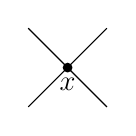
\begin{tikzpicture}[scale=0.5, transform shape]
			\draw (0,0) -- (2,-2);
			\draw (0,-2)-- (2,0);
			\node [circle,fill,inner sep=0.1pt,label=below:\huge$x$] at (1,-1) {x};
		\end{tikzpicture}
		=-i\lambda \int \dd^4 x$
   \item For each external point $ 
			\feynmandiagram[inline=(x.base),horizontal=x to y]{
				x[dot,label=$x$] -- y,
			}; = 1
			$
	\item Divide diagram by its symmetry factor $S$
\end{itemize}

Since the propagator $D_F(x-y) = \int \frac{\dd^4 p}{(2\pi)^4} \frac{i}{p^2 - m^2 + i\epsilon} e^{-ip(x-y)}$. It is actually simpler to express these in momentum space instead.

The way to do it is to asign a momentum $p$ to each propagator. (direction arbitrary)
\begin{center}
\feynmandiagram[horizontal=x to y]{
	x[dot,label=$x$] --[anti fermion,label=above$p$] y[dot, label=$y$],
};
\end{center}
\begin{itemize}
	\item assign $e^{ipy}$ to y-vertex (arrow out)
	\item assign $e^{-ipx}$ to x-vertex (arrow in)
	\item $\frac{i}{p^2-m^2+i\epsilon}$ to the line and the integration $\int \frac{\dd^4 p}{(2\pi)^4}$
\end{itemize}

At vertex $x$:
\begin{align*}
	\begin{tikzpicture}[baseline=(x)]
		\tikzfeynmanset{every vertex = dot,};
		\begin{feynman}
			\node (p1) at (0,0) {$p_1$};
			\node (p2) at (2,0) {$p_2$};
			\node (p3) at (0,-2) {$p_3$};
			\node (p4) at (2,-2) {$p_4$};
			\vertex (x) at (1,-1);
			\diagram*{
				(p1) --[fermion] (x),
				(p3) --[fermion] (x),
				(p4) --[anti fermion] (x),
				(x) --[anti fermion] (p2),
			};
		\end{feynman};
	\end{tikzpicture}
	&=-i\lambda \int \dd^4 x e^{-i(p_1 + p_2 + p_3)x + ip_4x} \\
	&= -i\lambda (2\pi)^4 \delta^{(4)} (p_1 + p_2 + p_3 - p_4)
\end{align*}
This imposes momentum conservation at vertex. $\delta^{(4)}$-functions make some of the momentum integrals trivial, always with $(2\pi)^4$ cancelled appropriately.

\paragraph{Momentum space Feynman rules}
\begin{itemize}
	\item Propagator $\feynmandiagram[inline=(x.base), horizontal=x to y]{x --[fermion, momentum=$p$] y}; = \frac{i}{p^2 - m^2 + i\epsilon}$
	\item Vertex (position integrated out) $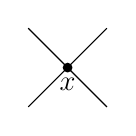
\begin{tikzpicture}[scale=0.5, transform shape]
			\draw (0,0) -- (2,-2);
			\draw (0,-2)-- (2,0);
			\node [circle,fill,inner sep=0.1pt,label=below:\huge$x$] at (1,-1) {x};
		\end{tikzpicture} = -i\lambda$ 
	\item External points $\begin{cases} e^{-ipx} & \text{incoming}\\ e^{+ipx}& \text{outgoing}\end{cases}$
		%%% TODO
	\item Impose momentum conservation at each vertex
	\item Integrate over each undetermined momentum $\int\frac{\dd^4 p}{(2\pi)^4}$
	\item Divided by symmetry factor
\end{itemize}

e.g.:
\begin{align*}
\feynmandiagram[inline=(a.base),small,horizontal=a to c]{
	a[dot,label=$x$] --[reversed momentum=$p$] b[dot,nudge up=1.65em] --[reversed momentum=$p$] c[dot,label=$y$];
	b --[half left, momentum=$q$] x [nudge up=1.5em] --[half left] b;
}; 
	=(-i\lambda) \int \frac{\dd^4 p}{(2\pi)^4}\frac{\dd^4 q}{(2\pi)^4} \left(\frac{i}{p^2-m^2+i\epsilon}\right)^2 \frac{i}{q^2-m^2+i\epsilon} e^{-ip(x-y)}
\end{align*}

\paragraph{Vacuum diagrams}
Disconnected pieces in Feynman diagrams are pretty bad. Not only $D_F(0) = \int \frac{\dd^4 p}{(2\pi)^4} \frac{i}{p^2 - m^2 + i\epsilon}$ is divergent (that will be taken care of later), it also contains an integral $\int \dd^4 x \,\text{const}$. Thus divergent once more!

Typical diagram contributing to 2-point function.
%TODO: diagrams
one piece connected to $x$ and $y$, plus disconnected pieces.

Call disconnected pieces $V_i \in \left\{	
	\feynmandiagram[layered layout,small, inline=(z.base),horizontal=x to z]{
			x --[opacity=0] y[dot] --[opacity=0] z;
			x --[half left] y --[half left] x;
			y --[half left] z --[half left] y;
			};		  \, ,\,
	\feynmandiagram[layered layout,small, inline=(z.base),horizontal=x to z2]{
			x --[opacity=0] y[dot] --[opacity=0] z[dot] --[opacity=0] z2;
			x --[half left] y --[half left] x;
			y --[half left] z --[half left] y;
			z --[half left] z2 --[half left] z;
			};		 \, , \,
	\dots
\right\}$. Points are connected internally, but not to external points.

$V_i$ can occur $n_i$-times, then 
\begin{align*}
	[\text{diagram}] = [\text{connected pieces}] \times \prod_{i} \frac{1}{n!} \left(V_i \right)^{n_i}
\end{align*}
The factorial is the symmetry factor of $n_i$ disconnected copies of $V_i$.

Then
\begin{align*}
	& \braket{0 | T \phi_1 \dots \phi_n S | 0} \\
	&= \sum_{\text{connected}} \; \sum_{\text{all}\{n_i\}} [\text{connected}] \times \prod_i \frac{1}{n_i !} (V_i)^{n_i}\\
   &= \left( \sum [\text{connected}] \right) \times \sum_{\text{all}\{n_i\}}\left( \prod_{i}\frac{1}{n_i !} (V_i)^{n_i} \right) \\
	& = \left( \sum [\text{connected}] \right) \times \prod_{i} \left( \sum_{n_i} \frac{1}{n_i !} (V_i)^{n_i} \right) \\
	& =\left( \sum [\text{connected}] \right) \times \exp(\sum_{i} V_i)
\end{align*}

Thus
\begin{align*}
	\text{sum of ALL diagrams} &= (\text{sum of all CONNECTED diagrams}) \\
								&\times \exp(\text{sum of all DISCONNECTED diagrams})
\end{align*}

Obvious from the above:
\begin{align*}
	\braket{0 | S | 0} = \braket{0 | T \{\exp(-\frac{i\lambda}{4!}\int \dd^4 x \phi^4(x))\}|0} = \exp(\text{sum of all vacuum bubbles})
\end{align*}

\paragraph{Conclusion} from the (unproven) formula for n-point correlation functions in the true, interacting vacuum:
\begin{align}
	\braket{\Omega | T \phi_1 \dots \phi_m | \Omega} &= \frac{ \braket{0 | T \phi_1 \dots \phi_m S |0}  }{ \braket{0 | S | 0}} \\
													 &= \sum \left( \text{connected diagrams with m external points} \right)
\end{align}
Here "connected" means connected to any external point. External points do not have to linked to each other.

\section{S-matrix elements and Feynman diagrams}
What is the correlation function in interacting vacuum $\braket{\Omega| T {\phi_1\dots\phi_m} | \Omega}$ good for? For scattering, shouldn't we rather look at $\braket{p_1 \dots p_m | S | p_A p_B}$
with the perturbative expansion of $S$ as before?

Decompose the S-matrix
\begin{align}
	S_{fi} = \delta_{fi} + i T_{fi} = \delta_{fi} + i(2\pi)^4 \delta^{(4)} (p_f-p_i)M_{fi}
\end{align}
$M_{fi}$ is the invariant matrix element, used to calculate cross section etc..

Zeroth term in the expansion of $S$
\begin{align*}
	\braket{ p_1 p_2 | p_A p_B} &= \sqrt{2E_1 2E_2 2E_A 2E_B} \braket{0 | a_1 a_2 a^+_A a^+_B | 0} \\
                               &= 2E_A 2E_B (2\pi)^6 \left( \delta^{(3)}(\pmb{p}_A-\pmb{p}_1) \delta^{(3)}(\pmb{p}_B - \pmb{p}_2) +   \delta^{(3)}(\pmb{p}_A-\pmb{p}_2) \delta^{(3)}(\pmb{p}_B - \pmb{p}_1)\right)
\end{align*}
This actually is "no scattering", part of the $\id$ in the S-matrix.

First term is 
\begin{align*}
	&\braket{p_1 p_2 | T \left( -\frac{i\lambda}{4!} \int \dd^4 x \phi^4(x) \right)|p_A p_B } \\
	&\stackrel{\text{wick}}{=} \braket{p_1 p_2 | :\left( -\frac{i\lambda}{4!} \int \dd^4 x \phi^4(x) + \text{contractions}\right ):|p_A p_B }
\end{align*}
However now the expectation value of a normal-ordered expression doesn't vanish!
\begin{align*}
	\phi^+(x) \ket{\pmb{p}} &= \int \frac{\dd^3 k}{(2\pi)^3 \sqrt{2E_k}} a_{\pmb{k}} e^{-ikx}\sqrt{2E_p} a^+_{\pmb{p}} \ket{0}\\
							&= \int \frac{\dd^3 k}{\sqrt{2E_k}} e^{-ikx}\sqrt{2E_p} \delta^{(3)}(\pmb{k}-\pmb{p}) \ket{0}\\
							&= e^{-ipx} \ket{0}
\end{align*}
So in general, need two field operators to annihilate the in-state and two field operators to create the out-states. We have new type of Feynman diagram to deal with external states. Define contractions of field operators with external states according to 
\begin{align*}
	\contraction{}{\phi}{(x)|}{\pmb{p}} \phi(x) \ket{\pmb{p}} &= e^{-ipx}\ket{0} \\
	\contraction{\langle}{\pmb{p}}{|\;}{\phi} \bra{\pmb{p}}\phi(x)  &= e^{+ipx}\ket{0} 
\end{align*}

How does this work for $p_A p_B \rightarrow p_1 p_2$ in $\phi^4$ at first order? It contains three types of terms: $\phi\phi\phi\phi$, $\contraction{}{\phi}{}{\phi}\phi\phi\phi\phi$ and $\contraction{}{\phi}{}{\phi}\phi\phi \contraction{}{\phi}{}{\phi}\phi\phi$ (fields without contraction are contracted with external states).

\begin{enumerate}
	\item 
		$\phi\phi\phi\phi$ allows full contractions with all external states. There is $4!$ possibilities
		\begin{align*}
				\begin{tikzpicture}[baseline=(x.base)]
				\begin{feynman}
					\vertex (x1) at (0,0) {$1$};
					\vertex (x2) at (1.5,0) {$2$};
					\vertex (x3) at (0,-2) {$A$};
					\vertex (x4) at (1.5,-2) {$B$};
					\vertex (x) at (0,-1);
					\diagram*{
						(x1) -- (x4);
						(x2) -- (x3);
					};
				\end{feynman}
			\end{tikzpicture}
			= 4! \frac{-i\lambda}{4!} \int \dd^4 x e^{-i(p_A + p_B - p_1 - p_2)x} = -i\lambda \underbrace{(2\pi)^4 \delta^{(4)}(p_A+p_B-p_1-p_2)}_\text{Pre-factor in definition of $i\mathcal{M}$}
		\end{align*}
		$i\mathcal{M}$ receives a contribution $-i\lambda$!
			\item 
		$\contraction{}{\phi}{}{\phi}\phi\phi\phi\phi$ leaves two operators to connect to external particles. Momentum conservation at each vertex. Still trivial!
		\begin{align*}
			\begin{tikzpicture}[baseline=(x.base)]
					\begin{feynman}
						\vertex (x1) at (0,0) {$1$};
						\vertex (x2) at (1.5,0) {$2$};
						\vertex (x3) at (0,-2) {$A$};
						\vertex (x4) at (1.5,-2) {$B$};
						\vertex (x) at (0,-1);
						\vertex (y) at (-0.5,-1);
						\diagram*[inline=(x.base)]{
							(x1) -- (x3);
							(x2) -- (x4);
							(x) --[half left] (y) --[half left] (x);
						};
					\end{feynman}
				\end{tikzpicture}
				+
				\begin{tikzpicture}[baseline=(x.base)]
					\begin{feynman}
						\vertex (x1) at (0,0) {$1$};
						\vertex (x2) at (1.5,0) {$2$};
						\vertex (x3) at (0,-2) {$A$};
						\vertex (x4) at (1.5,-2) {$B$};
						\vertex (x) at (1.5,-1);
						\vertex (y) at (1,-1);
						\diagram*{
							(x1) -- (x3);
							(x2) -- (x4);
							(x) --[half left] (y) --[half left] (x);
						};
					\end{feynman}
				\end{tikzpicture}
					+
				\begin{tikzpicture}[baseline=(x.base)]
					\begin{feynman}
						\vertex (x1) at (0,0) {$1$};
						\vertex (x2) at (1.5,0) {$2$};
						\vertex (x3) at (0,-2) {$A$};
						\vertex (x4) at (1.5,-2) {$B$};
						\vertex (a) at (0.5,-1.3);
						\vertex (b) at (0,-1);
						\diagram*{
							(x1) -- (x4);
							(x2) -- (x3);
							(a) --[half left] (b) --[half left] (a);
						};
					\end{feynman}
				\end{tikzpicture}
				+
				\begin{tikzpicture}[baseline=(x.base)]
					\begin{feynman}
						\vertex (x1) at (0,0) {$1$};
						\vertex (x2) at (1.5,0) {$2$};
						\vertex (x3) at (0,-2) {$A$};
						\vertex (x4) at (1.5,-2) {$B$};
						\vertex (a) at (1,-1.3);
						\vertex (b) at (1.5,-1);
						\diagram*{
							(x1) -- (x4);
							(x2) -- (x3);
							(a) --[half left] (b) --[half left] (a);
						};
					\end{feynman}
				\end{tikzpicture}
		\end{align*}
		Only fully connected Feynman diagrams contribute to $i T / i\mathcal{M}$!
	\item 
		\begin{align*}
			& -\frac{i\lambda}{4!} \int \dd^4 x \braket{p_1 p_2 | \contraction{}{\phi}{}{\phi} \phi\phi \contraction{}{\phi}{}{\phi} \phi\phi | p_A p_B } \\
			& = 	\feynmandiagram[layered layout,small, inline=(y.base),vertical=x to z]{
			x --[opacity=0] y[dot] --[opacity=0] z;
			x --[half left] y --[half left] x;
			y --[half left] z --[half left] y;
			}; \times 
			\left(
			\feynmandiagram[baseline=(y.base),small, horizontal=x1 to x2]{
				x1[label=$1$] --[opacity=0] x2 [label=$2$];
				x1 -- x3;
				x3[label=-90:A] --[opacity=0] x4[label=-90:B];
				x4 -- x2;
			}; 
			+ 
			\feynmandiagram[baseline=(y.base),small, horizontal=x1 to x2]{
				x1[label=$1$] --[opacity=0] x2 [label=$2$];
				x1 --[opacity=0] x3;
				x3[label=-90:A] --[opacity=0] x4[label=-90:B];
				x4 --[opacity=0] x2;
				x1 -- x4;
				x2 -- x3;
			};
		\right)
		\end{align*}
\end{enumerate}


%%%%%%%%%%%%%%%%%%%%%%%%%%%%%%%%%%%%%%%%%%%%%%%%%%%%%

\subsection{Feynman rules (with external lines)} 
\paragraph{Position space} calculate $iT$ by summing overall fully connected diagrams with
\begin{itemize}
	\item propagator 
		$\feynmandiagram[inline=(x.base),horizontal=x to y]{x [dot, label=$x$]  -- y [dot, label=$y$]}; = D_F(x-y)$
	\item vertex 
		$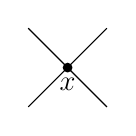
\begin{tikzpicture}[scale=0.5, transform shape]
			\draw (0,0) -- (2,-2);
			\draw (0,-2)-- (2,0);
			\node [circle,fill,inner sep=0.1pt,label=below:\huge$x$] at (1,-1) {x};
		\end{tikzpicture}
		=-i\lambda \int \dd^4 x$
	\item external lines "in" 
		$ 
		\feynmandiagram[inline=(x.base),horizontal=x to y]{
			x[dot,label=$x$] --[reversed momentum={\(p\)}] y,
		}; 
		= e^{-ip\cdot x}
		;\quad
		\feynmandiagram[inline=(x.base),horizontal=x to y]{
			x[dot,label=$x$] --[momentum={\(p\)}] y,
		};
		= e^{ip\cdot x}
		$
	\item divide diagram by its symmetry factor ${S}$
\end{itemize}

\paragraph{Momentum space} We have seen it before. Now (with external lines) all positions are integrated over. Result is a function of external momenta only. Integrating out all momentum-conserving $\delta$-distribution yields \underline{overall} momentum conservation: $(2\pi)^4 \delta^{(4)}(P_f - P_i)$

Momentum space Feynman rules for calculating $iM$:
\begin{itemize}
	\item internal propagator 
		$\feynmandiagram[inline=(x.base),horizontal=x to y]{x [dot, label=$x$]  -- y [dot, label=$y$]}; = \frac{i}{p^2 - M^2 + i\epsilon}$
	\item vertex 
		$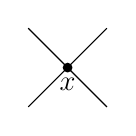
\begin{tikzpicture}[scale=0.5, transform shape]
			\draw (0,0) -- (2,-2);
			\draw (0,-2)-- (2,0);
			\node [circle,fill,inner sep=0.1pt,label=below:\huge$x$] at (1,-1) {x};
		\end{tikzpicture}
		=-i\lambda$
	\item external lines ("in" or "out") 
		$ 
		\feynmandiagram[inline=(x.base),horizontal=x to y]{
			x[dot,label=$x$] --[reversed momentum={\(p\)}] y,
		}; 
		= 1
		$
	\item impose 4-momentum conservation at each vertex
	\item integrate over all \underline{undetermined} momenta $\int \frac{\dd^4 p}{(2\pi)^4}$
	\item divide diagram by its symmetry factor ${S}$
\end{itemize}

There is still trouble in there. Consider the next-to-leading contribution to the scattering amplitude
\begin{align*}
	\begin{tikzpicture}[baseline=(y.base)]
	\begin{feynman}
		\vertex (x1) at (0,0) ;
		\vertex (x2) at (3,0) ;
		\vertex (x3) at (0,-3) ;
		\vertex (x4) at (3,-3) ;
		\vertex (y) at (1.5,-1.5);
		\vertex (a) at (2,-2);
		\vertex (b) at (2.5,-1.5);
		\diagram*{
			(x1) --[anti fermion, edge label=\(p_1\)] (y) --[anti fermion, edge label'=\(p'\)] (a) --[anti fermion, edge label'=\(p_B\)] (x4);
			(x2) --[anti fermion, edge label'=\(p_2\)] (y) --[anti fermion, edge label'=\(p_A\)](x3);
			(a) --[half left] (b) --[half left, anti fermion, edge label=\(k\)] (a);
		};
	\end{feynman}
	\end{tikzpicture}
	\begin{split}
	\quad = &\frac{1}{2} \int \frac{\dd^4 p'}{(2\pi)^4} \frac{i}{p'^2-m^2} \int \frac{\dd^4 k}{(2\pi)^4} \frac{i}{k^2-m^2} \\
	  &\times(-i\lambda)(2\pi)^4 \delta^{(4)}(p_A + p' - p_1 - p_2)\cdot (-i\lambda) (2\pi)^4 \delta^{(4)}(p_B-p')
	\end{split}
\end{align*}
This contains the internal propagator $\frac{i}{P^2_B-m^2+i\epsilon}$, but all the external particle are on their mass-shell, i.e.
\begin{align*}
	P^2_A = P^2_B = P^2_1 = P^2_2 = m^2 \; \Rightarrow \; \frac{i}{P^2_B - m^2} = \frac{i}{0}
\end{align*}

In addition to having \underline{fully connected} diagrams, also need to confine ourselves to \underline{amputated} diagrams: disregard all these diagrams with loops attached to external legs.
\begin{align*}
\begin{tikzpicture}[baseline=(y.base)]
\begin{feynman}
	\vertex (x4) at (3,-3) ;
	\vertex (y) at (1,-1);
	\vertex (a) at (2,-2);
	\vertex (b) at (2.7,-1.2);
	\diagram*{
		(y) --[anti fermion, edge label'=\(p\)] (a) --[anti fermion, edge label'=\(p\)] (x4);
		(a) --[half left] (b) --[half left] (a);
	};
\end{feynman}
\end{tikzpicture}
\begin{tikzpicture}[baseline=(y.base)]
\begin{feynman}
	\vertex (x4) at (3,-3) ;
	\vertex (y) at (1,-1);
	\vertex (x) at (2,-2);
	\vertex (a) at (1.6,-2.4);
	\vertex (b) at (2.8,-1.5);
	\diagram*{
		(y) --[anti fermion, edge label'=\(p\)] (x) --[anti fermion, edge label'=\(p\)] (x4);
		(a) --[half left] (b) --[half left] (a);
	};
\end{feynman}
\end{tikzpicture}\label{diagram:amputation}
\end{align*}

These diagrams represent the transition from the \underline{free} to the \underline{interacting asymptotic} states.

\paragraph{Lehmann-Symanzik-Zimmermann (LSZ) reduction formula} Proof on relation between correlation functions and S-matrix elements will be provided later.
\begin{align}
	\begin{split}
	&\prod_{i=1}^n \int \dd^4 x_i e^{ip_i \cdot x_i} \prod_{j=1}^{m} \int\dd^4 y_j e^{-i k_j \cdot y_i} \braket{\Omega | T\phi(x_1)\dots\phi(x_n)\phi(y_1)\dots\phi(y_m)|\Omega} \\
	&{=} (\text{disconnected stuff}) + \underbrace{\prod_{i=1}^n \frac{i\sqrt{Z}}{p_i^2 - m^2 +i\epsilon} \prod_{j=1}^m \frac{i\sqrt{Z}}{  _j^2 - m^2 + i\epsilon}}_{\text{remove poles from external legs}} \braket{p_1\dots p_n| S | k_i\dots k_m}
	\end{split}
\end{align}
$z$ is the wave-function renormalization factor.

Then amend Feynman rules above
\begin{center}
	consider only \underline{fully connected}, \underline{amputated} diagrams
\end{center}

\begin{align*}
	\braket{p_1 p_2 | iT | p_A p_B} &= 
\begin{tikzpicture}[scale=1, transform shape, baseline=(x.base)]
	\begin{feynman}
		\vertex (x1);
		\vertex (x2) at (2,0);
		\vertex (x3) at (0,-2);
		\vertex (x4) at (2,-2);
		\vertex (x) at (1,-1);
		\diagram*{
			(x1)-- (x) --(x2),
			(x3)-- (x) --(x4),
		};
	\end{feynman}
\end{tikzpicture}
+
	\begin{tikzpicture}[scale=1, transform shape, baseline=(x.base)]
	\begin{feynman}
		\vertex (x1);
		\vertex (x2) at (2,0);
		\vertex (x3) at (0,-2);
		\vertex (x4) at (2,-2);
		\vertex (xx) at (1,-0.6);
		\vertex (y) at (1,-1.4);
		\diagram*{
			(x1)-- (xx) --(x2),
			(x3)-- (y) --(x4),
			(xx) --[quarter left] (y) --[quarter left] (xx),
		};
	\end{feynman}
\end{tikzpicture}
+
\begin{tikzpicture}[scale=1, transform shape, baseline=(x.base)]
	\begin{feynman}
		\vertex (x1);
		\vertex (x2) at (2,0);
		\vertex (x3) at (0,-2);
		\vertex (x4) at (2,-2);
		\vertex (x) at (0.6,-1);
		\vertex (y) at (1.4,-1);
		\diagram*{
			(x1)-- (x) --(x3),
			(x2)-- (y) --(x4),
			(x) --[quarter left] (y) --[quarter left] (x),
		};
	\end{feynman}
\end{tikzpicture}
	+ \dots && \\
&+ \left(
\begin{tikzpicture}[scale=1, transform shape,baseline=(x.base)]
	\begin{feynman}
		\vertex (x1);
		\vertex (x2) at (2,0);
		\vertex (x3) at (0,-2);
		\vertex (x4) at (2,-2);
		\vertex (x)  at (2.5,-1);
		\vertex (y) at (2.5,-0.3);
		\vertex (z) at (2.5,-1.7);
		\diagram*{
			(x1)--(x2),
			(x3)--(x4),
			(x) --[half left] (y) --[half left] (x);
			(x) --[half left] (z) --[half left] (x);
		};
	\end{feynman}
\end{tikzpicture}
+ \dots \right) \quad && \text{yields} \ket{0} \rightarrow \ket{\Omega}\\
&+ \left( 
		\begin{tikzpicture}[baseline=(x.base)]
			\begin{feynman}
				\vertex (x) at (0.75, -1);
				\vertex (x1) at (0,0);
				\vertex (x2) at (1.5,0);
				\vertex (x3) at (0,-2);
				\vertex (x4) at (1.5,-2);
				\vertex (a) at (1,-1.3);
				\vertex (b) at (1.5,-1);
				\diagram*{
					(x1) -- (x4);
					(x2) -- (x3);
					(a) --[half left] (b) --[half left] (a);
				};
			\end{feynman}
		\end{tikzpicture}
		+ \dots
	\right) \quad && \text{yields} \ket{p}_{\text{free}} \rightarrow \ket{p}_{\text{int}}\\
&+ \left( 
\begin{tikzpicture}[baseline=(x.base)]
			\begin{feynman}
				\vertex (x1) at (0,0) {$1$};
				\vertex (x2) at (1.5,0) {$2$};
				\vertex (x3) at (0,-2) {$A$};
				\vertex (x4) at (1.5,-2) {$B$};
				\vertex (x) at (0,-1);
				\vertex (y) at (-0.5,-1);
				\diagram*[inline=(x.base)]{
					(x1) -- (x3);
					(x2) -- (x4);
				};
			\end{feynman}
		\end{tikzpicture}
+
	\begin{tikzpicture}[baseline=(x.base)]
			\begin{feynman}
				\vertex (x1) at (0,0) {$1$};
				\vertex (x2) at (1.5,0) {$2$};
				\vertex (x3) at (0,-2) {$A$};
				\vertex (x4) at (1.5,-2) {$B$};
				\vertex (x) at (0,-1);
				\vertex (y) at (-0.5,-1);
				\diagram*[inline=(x.base)]{
					(x1) -- (x3);
					(x2) -- (x4);
					(x) --[half left] (y) --[half left] (x);
				};
			\end{feynman}
		\end{tikzpicture}
		+ \dots
	\right) \quad &&\text{yields } \id \text{ in S-matrix}
\end{align*}

All allowed scattering diagrams $2 \rightarrow 2$ in $\phi^4$ up to $\mathcal{O}(\lambda^2)$:
\begin{align*}
	\begin{tikzpicture}[scale=1, transform shape, baseline=(x.base)]
	\tikzfeynmanset{every vertex = {dot},}
	\begin{feynman}
		\node (x1) {$p_1$};
		\node (x2) at (2,0) {$p_2$};
		\node (x3) at (0,-2) {$p_A$};
		\node (x4) at (2,-2) {$p_B$};
		\vertex (x)[dot] at (1,-1);
		\diagram*{
			(x1)-- (x) --(x2),
			(x3)-- (x) --(x4),
		};
	\end{feynman}
\end{tikzpicture}
+
	\begin{tikzpicture}[scale=1, transform shape, baseline=(x.base)]
	\tikzfeynmanset{every vertex = {dot},}
	\begin{feynman}
		\node (x1);
		\node (x2) at (2,0);
		\node (x3) at (0,-2);
		\node (x4) at (2,-2);
		\vertex (xx) at (1,-0.6);
		\vertex (y) at (1,-1.4);
		\vertex (s) at (1,-3) {$\color{red} s$};
		\diagram*{
			(x1)-- (xx) --(x2),
			(x3)-- (y) --(x4),
			(xx) --[quarter left] (y) --[quarter left] (xx),
		};
	\end{feynman}
\end{tikzpicture}
+
\begin{tikzpicture}[scale=1, transform shape, baseline=(x.base)]
	\tikzfeynmanset{every vertex = {dot},}
	\begin{feynman}
		\node (x1);
		\node (x2) at (2,0);
		\node (x3) at (0,-2);
		\node (x4) at (2,-2);
		\vertex (x) at (0.6,-1);
		\vertex (y) at (1.4,-1);
		\vertex (t) at (1,-3) {$\color{red} t$};
		\diagram*{
			(x1)-- (x) --(x3),
			(x2)-- (y) --(x4),
			(x) --[quarter left] (y) --[quarter left] (x),
		};
	\end{feynman}
\end{tikzpicture}
+
\begin{tikzpicture}[scale=1, transform shape, baseline=(x.base)]
	\tikzfeynmanset{every vertex = {dot},}
	\begin{feynman}
		\node (x2) at (0,0);
		\node (x1) at (2,0);
		\node (x3) at (0,-2);
		\node (x4) at (2,-2);
		\vertex (x) at (0.6,-1);
		\vertex (y) at (1.4,-1);
		\vertex (u) at (1,-3) {$\color{red} u$};
		\diagram*{
			(x1)--[quarter right] (x) --(x3),
			(x2)--[quarter left] (y) --(x4),
			(x) --[quarter left] (y) --[quarter left] (x),
		};
	\end{feynman}
\end{tikzpicture}
\end{align*}

Define the Lorentz-invariant quantities, \textit{Mandelstam variables}:
\begin{align}
	s = \left( p_A + p_B \right)^2, \quad t = \left( p_A - p_1 \right)^2, \quad u = \left( p_A - p_2 \right)^2
\end{align}

\begin{align*}
	\begin{tikzpicture}[scale=1, transform shape, baseline=(x.base)]
	\tikzfeynmanset{every vertex = {dot},}
	\begin{feynman}
		\node (x1) {$p_1$};
		\node (x2) at (2,0) {$p_2$};
		\node (x3) at (0,-2) {$p_A$};
		\node (x4) at (2,-2) {$p_B$};
		\vertex (xx) at (1,-0.5);
		\vertex (y) at (1,-1.5);
		\diagram*{
			(x1)-- (xx) --(x2),
			(x3)-- (y) --(x4),
			(xx) --[quarter left, anti fermion, edge label=\(-k\)] (y) --[quarter left, fermion, edge label=\(p_A + p_B + k\)] (xx),
		};
	\end{feynman}
\end{tikzpicture}
= \frac{1}{2} (-i\lambda)^2 \int \frac{\dd^4 k}{(2\pi)^4} \frac{i}{k^2 - m^2 + i\epsilon} \frac{i}{(p_A + p_B + k)^2 - m^2 +i\epsilon} \eqdef \frac{1}{2} (-i \lambda)^2 i J(s)
\end{align*}

Then the complete invariant amplitude is
\begin{align}
	M = - \lambda - \frac{\lambda^2}{2} \left( J(s) + J(t) + J(u) \right)
\end{align}

\section{Scattering cross section}\label{sec:croSec}
This section is based on Itzykson \& Zuber, Chapter 5.1. \\
The aim is to relate (differential) cross section to reduced/invariant matrix element $M_{fi}$. First we describe the initial states not as momentum eigenstates $\ket{p_A p_B}$, but as wave packets.
\begin{align*}
	\ket{i} = \int \frac{\dd^3 k_A}{(2\pi)^3 2k_A^0} \frac{\dd^3 k_B}{(2\pi)^3 2k_B^0} f(k_A) g(k_B) \ket{k_A k_B}
\end{align*}
with $f(k_A)$, $g(k_B)$ strongly peaked at $k_A \approx p_A$, $k_B \approx p_B$.

We can write the transition amplitude to the final state $\ket{f} \propto \ket{p_1 p_2}$ (note: normalisation not the same)
\begin{align*}
	A_{\textcolor{red}{f}i} &= \int \frac{\dd^3 k_A}{(2\pi)^3 2k_A^0} \frac{\dd^3 k_B}{(2\pi)^3 2k_B^0} f(k_A) g(k_B) \braket{\textcolor{red}{f} | iT | k_A k_B} \\
							&= \int \frac{\dd^3 k_A}{(2\pi)^3 2k_A^0} \frac{\dd^3 k_B}{(2\pi)^3 2k_B^0} f(k_A) g(k_B) (2\pi)^4 \delta^{(4)}(\underbrace{\textcolor{red}{p_f}}_{=p_1 + p_2}-k_A-k_B) i M(\textcolor{red}{f}, k_A,k_B) 
\end{align*}
Thus the \underline{transition probability}:
\begin{align*}
	\omega_{fi} &= (2\pi)^8 \int \frac{\dd^3 k_A}{(2\pi)^3 2k_A^0} \frac{\dd^3 k_B}{(2\pi)^3 2k_B^0} \frac{\dd^3 q_A}{(2\pi)^3 2q_A^0} \frac{\dd^3 q_B}{(2\pi)^3 2q_B^0} f(k_A) g(k_B) f(q_A)^* g(q_B)^*  \\
				&\times\qquad \underbrace{\delta^{(4)}(p_f-k_A-k_B)\delta^{(4)}(p_f-q_A-q_B)}_{=\delta^{(4)}(q_A+q_B-k_A-k_B)\delta^{(4)}(p_f-p_A-p_B)} \underbrace{M(\textcolor{red}{f}, k_A,k_B)  M^*(\textcolor{red}{f}, q_A,q_B)}_{\approx |M(f, p_A, p_B)|^2} \\
			\shortintertext{Using the fourier representation of delta function $\delta^{(4)}(q_A+q_B-k_A-k_B) = (2\pi)^{-4} \int \dd^4 x e^{i(k_A + k_B -q_A-q_B)\cdot x}$} \\
				&= \int \dd^4 x \underbrace{\int  \frac{\dd^3 k_A}{(2\pi)^3 2k_A^0}\frac{\dd^3 q_A}{(2\pi)^3 2q_A^0} e^{i(k_A - q_A)\cdot x} f(k_A) f^*(q_A)}_{\defeq |\tilde{f}(x)|^2} \\
				&\times \qquad \underbrace{\int \frac{\dd^3 k_B}{(2\pi)^3 2k_B^0} \frac{\dd^3 q_B}{(2\pi)^3 2q_B^0} e^{i(k_B-q_B)\cdot x} g(k_B)g^*(q_B)}_{\defeq |\tilde{g}(x)|^2} (2\pi)^4 \delta^{(4)}(p_f - p_A - p_B) \cdot |M(f, p_A, p_B)|^2 \\
				&\quad \shortintertext{Using Fourier transformation $\tilde{g}(x) \defeq \int \frac{\dd^3 q}{(2\pi)^3 2q^0} e^{iq\cdot x}g(q) $} \\
				& = \textcolor{blue}{\int \dd^4 x} \textcolor{purple}{|\tilde{f}(x)|^2} \textcolor{orange}{|\tilde{g}(x)|^2} (2\pi)^4 \delta^{(4)}(p_f - p_A - p_B) \cdot |M(f, p_A, p_B)|^2
\end{align*}
note that $M(f,p_A, p_B)$ and $M(p_1, p_2, p_A, p_B)$ have different normalisation.

We now consider transition probability per unit volume per unit time:
\begin{align*}
	\frac{\dd \omega_{fi}}{\textcolor{blue}{\dd V \dd t}} = \textcolor{purple}{\left( \text{incident flux} \right)} \cdot \textcolor{orange}{\left( \text{target density} \right)} \cdot \dd \sigma
\end{align*}
with $\dd \sigma$ the infinitesimal cross section for scattering into final state $\bra{f}$.

Product $\textcolor{purple}{\left( \text{incident flux} \right)} \cdot \textcolor{orange}{\left( \text{target density} \right)}$ denotes overlap of wave function. Necessary condition!

Covariant renormalization of states $\braket{\pmb{p} | \pmb{q}} \sim 2p^0 \delta^{3}(\pmb{p}-\pmb{q})$ means the number of particles per unit volume is $2p_A^0 |\tilde{f}(x)|^2$ and $2p_B^0 |\tilde{g}(x)|^2$, respectively.

Assume 
\begin{align*}
\begin{tikzpicture}[baseline=(a.base)]
	\tikzfeynmanset{every vertex = dot,};
	\begin{feynman}
		\vertex (a) at (0,0);
		\vertex (b) at (2,0) ;
	\node (c) at (2.7,0) {$\pmb{p}_B=0$};
		\diagram*{
		(a) --[fermion, edge label=\(p_A\)] (b);
	};
	\end{feynman}
\end{tikzpicture}
\end{align*}
in target rest frame. Then $2p_B^0 = 2m_B$ and $\textcolor{orange}{\text{target density}} = \textcolor{orange}{2m_B |\tilde{g}(x)|^2}$

Incident flux $= |\pmb{v}_A| \cdot 2 p_A^0 |\tilde{f}(x)|^2 = \textcolor{purple}{2 |\pmb{p}_A| |\tilde{f}(x)|^2}$ since $|\pmb{v}_A| = |\pmb{p}_A|/p_A^0$. Then 
\begin{align*}
	\dd \sigma  &= (2\pi)^4 \delta^{(4)}(p_f -p_A -p_B) \frac{1}{4m_B |\pmb{p_A}|} |M(f,p_A,p_B)|^2 \\
	\shortintertext{for $A+B \rightarrow 1+2$ processes}	\\
				&= \textcolor{red}{\int_{\Delta} \frac{\dd^3 p_1}{(2\pi)^3 2p^0_1} \frac{\dd^3 p_2}{(2\pi)^3 2p^0_2}} (2\pi)^4 \delta^{(4)}(\textcolor{red}{p_1 + p_2} - p_A - p_B)\frac{1}{4m_B |\pmb{p_A}|} |M(\textcolor{red}{p_1}, \textcolor{red}{p_2},p_A,p_B)|^2 
\end{align*}
with $\Delta$ energy-momentum resolution of 4-momentum of final state $\ket{f}$.

Covariant form of 
\begin{align}
	m_B \cdot |\pmb{p}_A| = m_B \sqrt{(p_A^0)^2 - m_A^2} = \sqrt{(p_A \cdot p_B)^2 - m_A^2 m_B^2} \eqdef F \label{math:F}
\end{align}

This is scattering into arbitrary final state subject to 4-momentum conservation: $p_A + p_B = p_1 + p_2$.

Consider now \underline{differential} cross section for scattering into a particular infinitesimal solid angle $\dd \Omega$, hence specific momentum $\dd p_1$, $\dd p_2$ variations:
\begin{align}
	\dd \sigma &= \frac{1}{4F}\prod_f \frac{\dd^3 p_f}{(2\pi)^3 2p_f^0} (2\pi)^4 \delta^{(4)}(p_A+p_B-\sum_f p_f)|M|^2 \notag \\
			   &\stackrel{f=1,2}{=}  \frac{1}{4F} \frac{\dd^3 p_1}{(2\pi)^3 2p_1^0} \frac{\dd^3 p_2}{(2\pi)^3 2p_2^0} (2\pi)^4 \delta^{(4)}(p_i- p_f)|M|^2 \notag\\
			   &= \frac{1}{64\pi^2 F} \frac{\dd^3 p_1}{E_1} \frac{\dd^3 p_2}{E_2} \delta^{(4)}(p_1 + p_2 - p_i) |M|^2 \notag\\
			   &\qquad \boxed{ 
				   \begin{array}{ll}
				   \int \frac{\dd^3 p_1}{E_1} \frac{\dd^3 p_2}{E_2} \delta^{(4)}(p_1 + p_2 - p_i)  \\ 
				   \stackrel{\text{CMS}}{=} \int \dd |\pmb{p}_1| \dd \Omega_1 \frac{|\pmb{p}_1|^2}{E_1 E_2} \delta (E_1 + E_2 -E_i) \\
				   = \int \dd (E_1 + E_2) \frac{\dd |\pmb{p}_1|}{\dd (E_1 + E_2)} \dd \Omega_1 \frac{|\pmb{p}_1|^2}{E_1 E_2} \delta (E_1 + E_2 -E_i)   \\
				   = \frac{|\pmb{p}_1|^2}{E_1 E_2} \left( \frac{|\pmb{p}_1|}{E_1} + \frac{|\pmb{p}_1|}{E_2} \right)^{-1} \dd \Omega_1 \\
				   = \frac{|\pmb{p}_1|\dd \Omega_1}{E_1 + E_2} =  \frac{|\pmb{p}_1|\dd \Omega_1}{E_i}
				   \end{array}
			   } \notag \\
			   &\frac{\dd \sigma}{\dd \Omega} = \frac{1}{64 \pi^2} \frac{|\pmb{p}_1|}{F\cdot E_i} |M|^2	
\end{align}

Rewrite all kinematic factors in terms of $s=(p_A+p_B)^2=(p_1+p_2)^2$. Define the function
\begin{align}
	\lambda(x,y,z) \defeq x^2 + y^2 +z^2 -2(xy + xz + yz)
\end{align}
then
\begin{align*}
	F &= \sqrt{(p_A\cdot p_B)^2 - m_A^2 m_B^2} = \frac{1}{2} \lambda^{\frac{1}{2}}(s,m^2_A,m^2_B) = \sqrt{s} |\pmb{p}_i| \\
	  &\qquad \boxed{ \begin{array}{ll}
			  \lambda (s,m_A^2, m_B^2) &= s^2 -2s(m_A^2 + m_B^2)-(m_A^2 - m_B^2)^2 =  (s - (m_A + m_B)^2)(s - (m_A - m_B)^2) \\
									   &= (2p_A \cdot p_B -2 m_A\cdot m_B) \cdot (2p_A \cdot p_B + 2 m_A\cdot m_B) = 4 \left[ (p_A p_B)^2 - m_A^2 m_B^2 \right]  \\
									   &\quad \boxed{ 
					   \begin{array}{ll}
						   p_A = (c\sqrt{s}, \pmb{p}_i),\, c \in [0,1] &\rightarrow m^2_A = c^2s - |\pmb{p}_i|^2 \\
						   p_B = ((1-c)\sqrt{s}, -\pmb{p}_i) &\rightarrow m^2_B = (1-c)^2 s - |\pmb{p}_i|^2
						\end{array}
					} \\
									   & =4 \left[ \left((c(1-c)s + p_i^2 \right)^2 + (c^2s - p_i^2)((1-c)^2s - p_i^2)\right] = 4 s |\pmb{p}_i|^2
	  \end{array} } \\
	|\pmb{p}_f| &= \sqrt{E^2_{1,2} - m_{1,2}^2} = \frac{1}{2\sqrt{s}} \lambda^{\frac{1}{2}}(s, m_1^2, m_2^2) \\
	E_i & = \sqrt{s}
\end{align*}

\begin{align}
	\frac{\dd \sigma}{\dd \Omega}_{CMS} = \frac{1}{64 \pi^2 s} \frac{|\pmb{p}_f|}{|\pmb{p}_i|}|M|^2 = \frac{1}{64\pi^2 s} \sqrt{\frac{\lambda(s, m_1^2, m_2^2)}{\lambda(s, m_A^2, m_A^2)}} |M|^2
\end{align}

Decay rate instead of cross section means no "incident flux" to divide by, only "target density"
\begin{align}
	\dd \Gamma = \frac{1}{2m_A} \prod_f \frac{\dd^3 p_f}{(2\pi)^3 2p_f^0} (2\pi)^4 \delta^{(4)}(p_A - \sum_f p_f) |M|^2
\end{align}

Particles with spin (unpolarized): sum over outgoing or average over initial spins
\begin{align}
	|M|^2 \rightarrow \frac{1}{(2s_A + 1)(2s_B + 1)} \sum_{s_i, s_f} |M_{fi}|^2
\end{align}

Symmetry factor $|M|^2 \rightarrow \frac{1}{s} |M|^2$ with $s = \prod_i k_i!$ if there are $k_i$ identical particles of species $i$ in the final states.

If $1$ and $2$ are identical, then factor $\frac{1}{s} = \frac{1}{2}$ on the right hand side.

%%%%%%%%%%%%%%%%%%%%%%%%%%%%%%%%%%%%%%%%%
\section{Feynman rules for fermions}
Consider the simplest interacting theory with fermions, Yukawa-theory. We will treat QED later.
\begin{align}
	\lag = \frac{1}{2} \partial_\mu \phi \partial^\mu \phi - \frac{M^2}{2}\phi^2 + \bar{\psi} (i\slashed{\partial} - m) \psi -  g \bar{\psi} \psi \phi
\end{align} 

Feynman rules will involve:
\begin{itemize}
	\item scalar $\feynmandiagram[small, horizontal=a to b]{a[dot, label={\(x\)}] --[scalar] b[dot, label={\(y\)}];}; = D_F(x-y) = \int \frac{\dd^4}{(2\pi)^2} \frac{i}{p^2 - M^2 + i \epsilon} e^{-ip(x-y)}$
	\item fermions $\feynmandiagram[small, horizontal=a to b]{a[dot, label={\(x, \alpha\)}] -- [anti fermion] b[dot, label={\(y, \beta\)}];}; = S_F(x-y)_{\alpha \beta} = \int \frac{\dd^4}{(2\pi)^4} \frac{i(\slashed{p}+m)}{p^2 - m^2 + i\epsilon} e^{-ip(x-y)}$
	\item vertices $\feynmandiagram[baseline=(x.base),small, horizontal=x to c]{a--x[dot]; b--x; x--[scalar]c;}; = -ig\int \dd^4 x$
\end{itemize}

What previous steps need reconsideration due to the \underline{anti-commutating} fermion operators? Interaction Hamiltonian $\sim \bar{\psi}\psi \phi$ and in general compose of \underline{even} number of fermion fields (spin conservation and fermion number conservation). Thus there is no problem with time-ordered exponential in definition of S-matrix. (Time ordering always takes two or even number of fields.)

Remember the relation
\begin{align}
	T(\psi_\alpha(x) \bar{\psi}_\beta(x)) = \textcolor{red}{-} \bar{\psi}_\beta (x) \psi_\alpha(x) \text{ when } y^0 > x^0
\end{align}
Similarly in normal product: 
\begin{align}
	:\psi^+ \psi^-: = \textcolor{red}{-} \psi^- \psi^+
\end{align}
Then Wick's theorem is formally the same as before
\begin{align*}
	T(\psi_\alpha(x) \bar{\psi}_\beta(x)) = :\psi_\alpha(x) \bar{\psi}_\beta(x): + \contraction{}{\psi}{_\alpha(x)}{\bar{\psi}} \psi_\alpha(x) \bar{\psi}_\beta(x)
\end{align*}
note by definition $\contraction{}{\psi}{}{\psi} \psi\psi = \contraction{}{\bar{\psi}}{}{\bar{\psi}}\bar{\psi}\bar{\psi} = 0$

Thus contractions inside normal-ordered products would be
\begin{align*}
	:\psi_1 \psi_2 \bar{\psi}_3 \bar{\psi}_4:= \textcolor{red}{-} \contraction{}{\psi}{_1}{\bar{\psi}}\psi_1\bar{\psi}_3 :\psi_2 \bar{\psi}_4: = \textcolor{red}{-} S_F(x_1 - x_3) :\psi_2 \bar{\psi}_4:
\end{align*}
because of the additional operator exchange.

We will want to consider fermion-(anti-)fermion scattering. Leading contribution at $\mathcal{O}(g^2)$:
\begin{align*}
	\frac{1}{2!} (-ig)^2 \int \dd^4 x \dd^4 y \braket{p', k' |T\bar{\phi}(x) \phi(x) \phi(x) \bar{\phi}(y)\phi(y)|p,k}
\end{align*}

Contractions with initial-/final-state fermions?
\begin{align*}
	\phi^+(x) \ket{p,s} &= \int \frac{\dd^3 k}{(2\pi)^3 \sqrt{2E_k}} \sum_r a^r_k u_r(k) e^{-ik\cdot x} \sqrt{2E_p} a^{s\dagger}_p \ket{0} \\
						&= e^{-ip\cdot x} u_s(p) \ket{0}	
\end{align*}

So define
\begin{align}
	\begin{split}
	\contraction{}{\psi}{(x)|}{p,s} \psi(x) \ket{p,s} &=  e^{-ip\cdot x} u_s(p) \\
	\contraction{\langle}{p,s}{|\;}{\bar\psi} \bra{p,s}\bar\psi(x)  &=  e^{ip\cdot x} \bar{u}_s(p)
	\end{split}
\end{align}

Note, though, for \underline{anti-fermion states} $\ket{p', s'}$:
\begin{align}
	\begin{split}
	\contraction{}{\bar{\psi}}{(x)|}{p',s'} \bar{\psi}(x) \ket{p,s} &=  e^{-ip' \cdot x} \bar{v}_{s'}(p') \\
	\contraction{\langle}{p',s'}{|}{\psi} \bra{p',s'}\psi(x)  &=  e^{ip'\cdot x} v_{s'}(p')
	\end{split}
\end{align}

In short $\contraction{}{\psi}{|}{\;} \psi \ket{\;} $ contracts with a fermion, $\contraction{\langle}{\,\;}{|}{\psi} \bra{\;}\psi$ with an anti-fermion; vice verse for $\bar{\psi}$.

\paragraph{Momentum space Feynman rule for $iM$}
\begin{itemize}
	\item internal propagators 
		$$\feynmandiagram[small, horizontal=a to b]{a --[charged scalar, edge label={\(q\)}]b;};
		=\frac{i}{q^2 - M^2 + i\epsilon}$$
		$$\feynmandiagram[small, horizontal=a to b]{a[label={\(\beta\)}] --[edge label={\(q\)}, fermion]b[label={\(\alpha\)}];};
		=\frac{i(\slashed{p}+m)_{\alpha\beta}}{p^2-m^2+i\epsilon}$$
	\item vertex 
		$$\feynmandiagram[baseline=(x.base),small, horizontal=x to c]{a[label={\(\beta\)}]--[anti fermion] x[dot]; b[label={\(\alpha\)}]--[fermion]x; x--[scalar]c;}; = -ig\int \dd^4 x
		=ig\delta_{\beta\alpha}$$
	\item external lines
		\begin{itemize}
			\item "in" and "out" scalar 
				$\feynmandiagram[baseline=(x.base),small, horizontal=x to c]{a--[anti fermion] x[dot]; b--[fermion]x; x--[anti charged scalar, edge label={\(q\)}]c;}; = 
\feynmandiagram[baseline=(x.base),small, horizontal=c to x]{a--[anti fermion] x[dot]; b--[anti fermion]x; x--[charged scalar, edge label={\(q\)}]c;};
				= 1$
			\item "in"-fermion $\feynmandiagram[baseline=(x.base),small, horizontal=x to b]{a--[anti fermion] x[dot]; b--[fermion, edge label={\(p\)}]x; x--[scalar]c;};=u_s(p)$ and "out" fermion $\feynmandiagram[baseline=(x.base),small, horizontal=b to x]{a--[fermion] x[dot]; b--[anti fermion, edge label={\(p\)}]x; x--[scalar]c;};=\bar{u}_s(p)$
			\item "in"-anti-fermion $\feynmandiagram[baseline=(x.base),small, horizontal=x to b]{a--[fermion] x[dot]; b--[anti fermion, momentum={\(k\)}]x; x--[scalar]c;};=\bar{v}_s(k)$ and "out" anti-fermion $\feynmandiagram[baseline=(x.base),small, horizontal=b to x]{a--[anti fermion] x[dot]; b--[fermion, momentum={\(k\)}]x; x--[scalar]c;};={v}_s(k)$
		\end{itemize}
	\item impose energy-momentum conservation at each vertex 
	\item integrate over undetermined (loop) momenta 
	\item include an overall sign for the diagram
\end{itemize}

\paragraph{Note}
\begin{itemize}
	\item \underline{Arrows} on the fermion lines by convention denote \underline{fermion} (or charge) \underline{flow}. They must flow consistently through the diagram. ($\equiv$ fermion number conservation) (Only potential confusion: external anti-fermion lines)
	\item No symmetry factors (except vacuum bubbles \feynmandiagram[small, baseline=(a.base), horizontal=a to b]{a--[scalar]b; a--[anti fermion, half right]b; b--[anti fermion, half right] a;}; $\frac{1}{s} = \frac{1}{2}$). $\bar\psi \psi \phi$ allows for unambiguous contractions.
	\item Dirac indices are summed over at each vertex
		\begin{align*}
			\lag_\text{int} \approx \bar{\psi}_\alpha(x) \psi_\alpha(x) \phi(x)
		\end{align*}
		$(\slashed{p}+m)$ terms in propagator are matrix-multiplied contracted with external spinors, e.g.
		\begin{align*}
			\feynmandiagram[layered layout, small, baseline=(c.base), horizontal = a to b]{
				a --[anti fermion, edge label={\(p_3\)}] b;
				b --[anti fermion, edge label={\(p_2\)}] c;
				c --[anti fermion, edge label={\(p_1\)}] d;
				d --[anti fermion, edge label={\(p_0\)}] e;
				x --[scalar] b;
				y --[scalar] c;
				z --[scalar] d;
			};
			\sim \bar{u}_\alpha(p_3) \frac{i(\slashed{p}+m)_{\alpha\beta}}{p^2_2 - m^2 + i\epsilon} \frac{i(\slashed{p}+m)_{\beta\gamma}}{p^2_1 - m^2 + i\epsilon} u_{\gamma}(p_0)
		\end{align*}
	\item closed fermion loop
		\begin{align*}
			\feynmandiagram[layered layout, small, horizontal=y to x,baseline=(y.base)]{
				a --[scalar] y[dot, label=120:{\(y\)}];
				y --[fermion, half left] x[dot, label=30:{\(x\)}];
				x --[fermion, half left] y;
				x --[scalar] b;
			}; 
			&\sim \contraction{}{\bar{\psi}}{_{\alpha} (x) \psi_{\alpha} (x) \bar{\psi}_{\beta} (y)}{\psi} 
			\contraction{\bar{\psi}_{\alpha} (x) }{\psi}{_{\alpha} (x) }{\bar{\psi}}
			\bar{\psi}_{\alpha} (x) \psi_{\alpha} (x) \bar{\psi}_{\beta} (y) \psi_{\beta} (y) 
			= \textcolor{red}{-}\contraction{}{\psi}{_{\alpha} (x) }{\bar{\psi}} {\psi}_{\alpha} (x) \bar{\psi}_{\beta} (y) 
			\contraction{}{\psi}{_{\alpha} (x) }{\bar{\psi}} \psi_{\alpha} (x) \bar{\psi}_{\beta} (y) \\
			& = \textcolor{red}{-} S_F(y-x)_{\beta\alpha} S_F(x-y)_{\alpha\beta} 
			= \textcolor{red}{-} \textcolor{red}{\text{Tr}} \left( S_F(y-x) S_F(x-y) \right)
		\end{align*}
		It always (also with more propagators/couplings) involves an overall $\textcolor{red}{(-1)}$ and a trace $\textcolor{red}{\text{Tr}}(\dots)$.
\end{itemize}

\paragraph{Examples}
\begin{itemize}
	\item fermion-fermion scattering to lowest order $\mathcal{O}(g^2)$
		\begin{align*}
			iM &= \feynmandiagram[small, horizontal=x to y, baseline=(x.base)]{
				a--[anti fermion, edge label={\(p'\)}] x[dot];
				b--[fermion, edge label={\(p\)}] x;
				x--[scalar]y[dot];
				y--[fermion,edge label={\(k'\)}]c;
				y--[anti fermion, edge label={\(k\)}]d;
			};
			+
			\begin{tikzpicture}[scale=0.6, baseline=(a.base)]
				\begin{feynman}
					\diagram[horizontal'=a to b] {
				i1 [label=\(p\)]-- [fermion] a-- [draw=none] f1 [label=\(p'\)],
				a -- [scalar] b,
				i2 [label=\(k\)]-- [fermion] b-- [draw=none] f2 [label=\(k'\)],
				};
				\diagram* {
					(a) -- [fermion] (f2),
					(b) -- [fermion] (f1),
				};
				\end{feynman}
			\end{tikzpicture}\\
			   &= (-ig)^2 \left\{ \bar{u}(p')u(p) \frac{i}{\underbrace{(p'-p)^2}_{t}-M^2+i\epsilon} \bar{u}(k')u(k) \textcolor{red}{-} \bar{u}(p')u(k) \frac{i}{\underbrace{(p'-k)^2}_{u}-M^2+i\epsilon} \bar{u}(k') u(p) \right\}
		\end{align*}
	\item fermion-anti-fermion scattering
		\begin{align*}
			\feynmandiagram[small, horizontal=x to y, baseline=(x.base)]{
				a--[anti fermion] x[dot];
				b[particle=\(f\)]--[fermion] x;
				x--[scalar]y[dot];
				y--[anti fermion]c;
				y--[fermion]d[particle=\(\bar{f}\)];
			};
			+
			\feynmandiagram[small, vertical=x to y, baseline=(y.base)]{
				a--[fermion] x[dot];
				b--[anti fermion] x;
				x--[scalar]y[dot];
				y--[fermion]c[particle=\(\bar{f}\)];
				y--[anti fermion]d[particle=\(f\)];
			};
		\end{align*}
		These are tree diagrams. Thus there is no undetermined momenta to integrate.
\end{itemize}
